% !Mode:: "TeX:UTF-8"
%!TEX program  = xelatex

%\documentclass{cumcmthesis}
\documentclass[withoutpreface,bwprint]{cumcmthesis} %去掉封面与编号页
%\usepackage{diagbox}
\usepackage{url}
\title{ }
\tihao{B}
\baominghao{4321}
\schoolname{**大学}
\membera{A}
\memberb{B}
\memberc{C}
\supervisor{老师}
\yearinput{2018}
\monthinput{07}
\dayinput{16}

\begin{document}
	\title{高压油管的压力控制}
	
	\maketitle
	
	\begin{abstract}
		
		
		
		
		\keywords{\quad  \quad   \quad  }
	\end{abstract}
	
	
	
	
	%目录
	%\tableofcontents
	
	%\newpage
	\section{问题重述}
	%为何研究高压油管的压力控制
	燃油喷射系统由喷油泵、高压油管和喷油嘴等组成,是柴油机燃料的供给来源,被认为是柴油机的“心脏”。高压油管是燃油从喷油泵输送到喷油器的重要通道,其正常工作是保证发动机高效率工作的因素之一。高压油管一般采取多次喷射,能有效改善柴油机的排放性和燃油经济性。而燃油多次、间歇性进入和喷出会导致高压油管内产生压力波动,使得喷出的燃油量出现偏差,燃油量供应不足将显著影响柴油机的工作效率。因此,应设计合理的喷油泵与喷油器的工作机制以确保管内压力尽可能稳定。
	
	
	
	\subsection{问题的提出}
	问题一:对于某一特定的高压油管,通过单向阀开关控制向高压油管供油时间的长短,通过喷油器的开关控制向外的喷油量。问题一从相对简单的燃油进出特性开始考虑,设置单向阀每打开一次后就要关闭10$ms$,喷油嘴每秒工作10次,每次工作时喷油时间为2.4$ms$。在喷油孔周期性工作的情况下,要求设置合理单向阀开启时间以确保高压油管内压力尽可能保持在100MPa;调整开启时长使高压油管内的压力从100MPa通过2$s$、5$s$或10$s$增加到150MPa。
	
	
	问题二:调整燃油进出特性,考虑进油由高压油泵的柱塞控制,喷油由喷油嘴的针阀控制,喷油嘴与问题一中有相同的工作特性。高压油泵的压油由凸轮驱动,设置合理的凸轮角速度,使高压油管内的压力在整个工作进程中尽量稳定在100MPa。
	
	
	问题三:考虑较为复杂的情况,增加一个与问题一规律相同的喷油嘴和一个单向减压阀。减压阀可以使高压油管内的燃油在压力下回流到外部低压油路中。要求设计高压油泵与减压阀的控制方案。
	
	\section{模型的假设}
	在喷射过程计算中,考虑喷射过程的全部因素是不切实际的,为了研究该具体情况高压油管的喷射过程,做出适当假定,以建立简明的计算模型。
	\begin{itemize}
		\item 假设单向阀和喷油嘴周期性工作;在每一周期内,工作时间相同
		\item 忽略高压油管接口处的集中容积、油管变截面等对喷射过程的影响
		\item 喷油压力变化所引起的温度变化是微小的\cite{bib:one},因此不考虑温度随压力和时间的变化
		\item 假定燃油在各腔中静止压缩、膨胀,状态变化瞬间到达平衡,在同一时刻,各腔内压强处处相等
		\item 不考虑油管的燃油在泵、嘴两端接口处的流动损失
		
	\end{itemize}
	
	\section{符号说明}
	\begin{center}
		\begin{table}[!ht]
			\caption{符号说明}
			\centering
			\begin{tabular}{cc}
				\toprule[1.5pt]
				\makebox[0.3\textwidth][c]{符号}	&  \makebox[0.4\textwidth][c]{意义} \\ \midrule
				$P_c$ & 高压油管内平均压强 \\ 
				$P_p$ & 高压油泵内的平均压强 \\ 
				$Q_{in}$ & 进入高压油管的流量 \\
				$Q_{out}$ & 喷出高压油管的流量 \\ 
				$Q_{P}$ & 高压油泵的几何供油率 \\
				$Q_{VP}$ &  柱塞腔压力变化所引起的压缩油量变化率\\
				$\rho$ & 燃油的密度 \\
				$C$ & 燃油的流量系数 \\
				$E$ & 燃油的弹性模量 \\ 
				$L$ & 高压油腔内腔长度 \\
				$d_p$ & 柱塞腔内直径 \\
				$d_c$ & 高压油腔内直径 \\
				$d_v$ & 针阀直径 \\
				$d_{out}$ & 喷油器喷孔直径 \\
				$h_p$ & 柱塞升程 \\
				$h_v$ & 针阀升程 \\
				$A_c$ & 高压油管横截面积 \\
				$A_p$ & 柱塞腔横截面积 \\
				$A_{in}$ & 入口供油处横截面积 \\
				$A_{out}$ & 出口喷油处横截面积 \\
				$V_c$ & 高压油管内腔容积 \\
				$V_p$ & 柱塞腔横截面积 \\  \bottomrule[1.5pt]
			\end{tabular}
		\end{table}
	\end{center}
	
	\section{问题分析}
	由于燃油是可压缩流体,燃油进入和喷出将会高压油管内的燃油密度,而压强的变化量与密度变化量成正比。为了使压力尽可能稳定在100MPa,根据假设4,即尽量使平均压强变化量为0。因此要通过进出流量、密度和弹性模量建立压强与时间之间的关系。
	在问题一中,进入高压油管的流量与A小孔两边的压力有关;喷出的流量由喷油速率示意图可以确定。
	
	
	在问题二中,由于单向阀的开关不再随时间固定的开闭,而由单向阀两边的压力决定,因此进入高压油管的燃油量由凸轮的轮动有关;喷出的流量由喷油嘴的针阀上下运动决定。凸轮轮动使高压油泵的体积变化,进而影响燃油的密度和压力,当燃油压力大于高压油管内的燃油压力时,单向阀开启,燃油从高压油泵流入高压油管,从而影响高压油管的压力。凸轮转动只由凸轮的角速度决定,因此,应建立模型体现压力与凸轮角速度的关系和时间的关系。
	
	
	在问题二基础上,增加一个减压单向阀和喷油嘴,只需调整问题二的模型。
	
	
	\section{模型的建立与解决}
	\subsection{问题一:阀-管-喷嘴模型}
	在问题一中,根据题目所给条件,只需考虑单向阀流入高压油管的燃油量与喷出的燃油量,而流入与喷出的燃油将影响高压油管内的燃油密度,进而影响管内压力,因此我们将把高压油管、单向阀与喷油嘴看作一个系统,研究该系统内压力的变化,期望建立压力与时间的变化方程。
	
	我们假设该系统在开始工作后,单向阀与喷油嘴立即投入工作,两者工作相互独立。喷油嘴1s内工作十次,我们假设了喷油嘴为周期性喷油,于是可以确定其工作周期。系统内有可能出现喷油嘴与单向阀同时开启、一开一闭以及同时关闭等四种状态,由于通过两者的燃油流量只由压力差和小孔面积决定,因此可以将单向阀和喷油嘴的工作状态看作相互独立,那么就不需要考虑不同状态带来的对阀和嘴的影响。
	\subsubsection{公式推导}
	根据燃油的可压缩性,在高压油管与外界没有质量交换时,其内的压强变化为
	\begin{equation}
	E = -\frac{\mathrm{d}P_c}{\mathrm{d}V}V
	\end{equation}
	其中:$V$代表高压油管内的体积,符号表示压强随着体积的增大而减小。
	当单向阀和喷油嘴开启时,进出高压油管的流量为
	\begin{equation}
	Q = CA\sqrt{\frac{2\Delta P}{\rho}}
	\end{equation}
	其中:$C = 0.85$为流量系数,$A$为小孔的面积,$\Delta P$为小孔两边的压力差,$\rho$为高压侧燃油的密度。
	
	进入高压油管的燃油量与A处的单向闸开启时间有关,假设单向闸在工作周期开始时便开启,设开启时间为$\widetilde{t}$,记工作周期为$T_{in} = 10ms + \widetilde{t}$那么进入高压油管的流量为:
	\begin{equation}
	Q_{in} = \left\{ 
	\begin{array}{ll}
	CA\sqrt{\frac{2(P_c-P_p)}{\rho_c}}&,nT_{in}\leq t <nT_{in} + \widetilde{t} \\
	0&,nT
	-{in}+\widetilde{t}\leq t <(n+1)T_{in}
	\end{array}
	\right.
	\end{equation}
	$n = 1,2,3,...$
	
	对喷油嘴,假设喷油嘴在一个工作周期开始时便开启,记工作周期为$T_{out} = 10 ms$。由题目所给喷油速率$(mm^3)$与时间$(ms)$的关系可知喷油流量为
	\begin{equation}
	Q_{out} = \left\{ 
	\begin{array}{ll}
	100t&,nT_{out}\leq t<nT_{out}+0.2 \\
	20&,nT_{out}+0.2\leq t< nT_{out}+2.2\\
	-100t+240&,nT_{out}+0.2\leq t< nT_{out}+2.4\\
	0&,nT_{out}+2.4\leq t <(n+1)T_{out}
	\end{array}
	\right.
	\end{equation}
	$n = 1,2,3,...$
	
	因此,当高压油管与外界有质量交换时,压力控制结合(3)-(4)对方程(1)变形为$\frac{\mathrm{d}P}{\mathrm{d}t}=-\frac{E}{V}\frac{\mathrm{d}V}{\mathrm{d}t}$,其中$\frac{\mathrm{d}V}{\mathrm{d}t}$考虑进入与流出腔体的流量。于是得到了高压油管内压力变化量与时间的关系:
			\begin{equation}
			\frac{\mathrm{d}P_c}{\mathrm{d}t} = \frac{E}{V_c}(Q_{in} - Q_{out})
			\end{equation}
			
			该方程也即为可压缩流体的连续性方程,为我们的目标方程。然而,在此式中弹性模量与密度都是与压强有关的,因此要先得到两者与压强的表达式。
			\subsubsection{弹性模量与压强的关系}
			根据附件三所给的数据,我们可以通过函数拟合得到弹性模量与压强之间的关系为:
			\begin{equation}
			E = 1489 e^{0.00284P} + 48.79 e^{0.01376 P}
			\end{equation}
			拟合误差为 再搞张图
			
			
			\subsubsection{燃油压强与燃油密度的关系}
			燃油的压力变化量与密度变化量成正比,比例系数为$\frac{E}{\rho}$,其中$E$为弹性模量,因此可列出常微分方程:
			\begin{equation}
			\frac{\mathrm{d}P}{\mathrm{d}\rho} = \frac{E}{\rho} = \frac{1489 e^{0.00284P} + 48.79 e^{0.01376 P}}{\rho}
			\end{equation}
			已知方程的边值条件为$P = 100MPa, \rho = 0.850\ mg/mm^3$,同时带入公式(6),可解得燃油压强与密度的表达式。
			\subsection{模型一求解}
			在第一问中,我们期待找到适合的$\widetilde{t}$,使微分方程公式(5)的解稳定后的平均值为100$MPa$且方差较小。
			在第二问中,要求将高压油管内的压强从100MPa增加到150MPa,我们将设计单向阀时长调整方案,调整方案分为两个阶段,第一阶段,增长单向阀时长使高压油管增加到150MPa;第二阶段,降低单向阀时长使高压油管稳定在150MPa。
			\subsubsection{基于四阶龙格库塔的数值仿真}
			对于复杂的常微分方程常常难以得到解析解,因此我们选择使用合理的微分方程数值解法,从而得到随着时间变化高压油管内平均压强的变化。龙格-库塔算法是一种流行的高精度数值方法,最常用的为经典四阶龙格-库塔算法($classical\ fourth-order\ RK\ method$),其形式为:
			\[
			y_{n+1}=y_{n}+\frac{1}{6}(k_{1}+2k_{2}+2k_{3}+k_{4})h
			\]
			
			其中:
			\begin{align*}
			k_{1}&=f(t_{i},y_{i})\\
			k_{2}&=f(t_{i}+\frac{1}{2}h,y_{i}+\frac{1}{2}hk_{1})\\
			k_{3}&=f(t_{i}+\frac{1}{2}h,y_{i}+\frac{1}{2}hk_{2})\\
			k_{4}&=f(t_{i}+h,y_{i}+hk_{3})
			\end{align*}
			
			$h$为时间步长
			\subsubsection{情况一:恒定稳定压强的求解}
			结合公式(3)-(6),再加上高压油管内容积,常微分方程表示为:
			\begin{equation} \left\{
			\begin{aligned}
			&\frac{\mathrm{d}P_c}{\mathrm{d}t} = \frac{E}{V_c}(Q_{in} - Q_{out}) \\
			&Q_{in} (P_c,t) \\
			&Q_{out} (P_c,t) \\
			&E(P_c) = E = 1489 e^{0.00284P_c} + 48.79 e^{0.01376 P_c} \\
			&V_c = A_cL = \frac{\pi d_p^2}{4} \cdot L
			\end{aligned}
			\right. \end{equation}
			初值条件为$t = 0, P_c = 100MPa$
			
			
			首先,我们任意给定了单向阀的开启时间$\widetilde{t}$,取时间步长$\delta t = 0.01ms$,对上述方程利用四阶龙格库塔法解出数值解。可以得到阀-管-嘴系统平衡后高压油管内的平均压强。然后,用二分法调整$\widetilde{t}$确定单向阀的开启时间,使平均压强在100MPa左右的大致范围,得到大致范围是$\widetilde{t}\in [0.29ms,0.3ms]$。
			
			在该区间内,取较小步长,用MATLAB得到不同$\widetilde{t}$时的方差与平均值,如图1所示。可以看到在该区间内去不同的值,平均值变化微小,而方差在$\widetilde{t}=0.296$时达到最小,因此我们确定单向阀周期性工作,开启$0.296s$后停止工作启$10s$可以使高压油管内平均压强稳定在100MPa。
			\begin{figure}[!htbp]
				\centering
				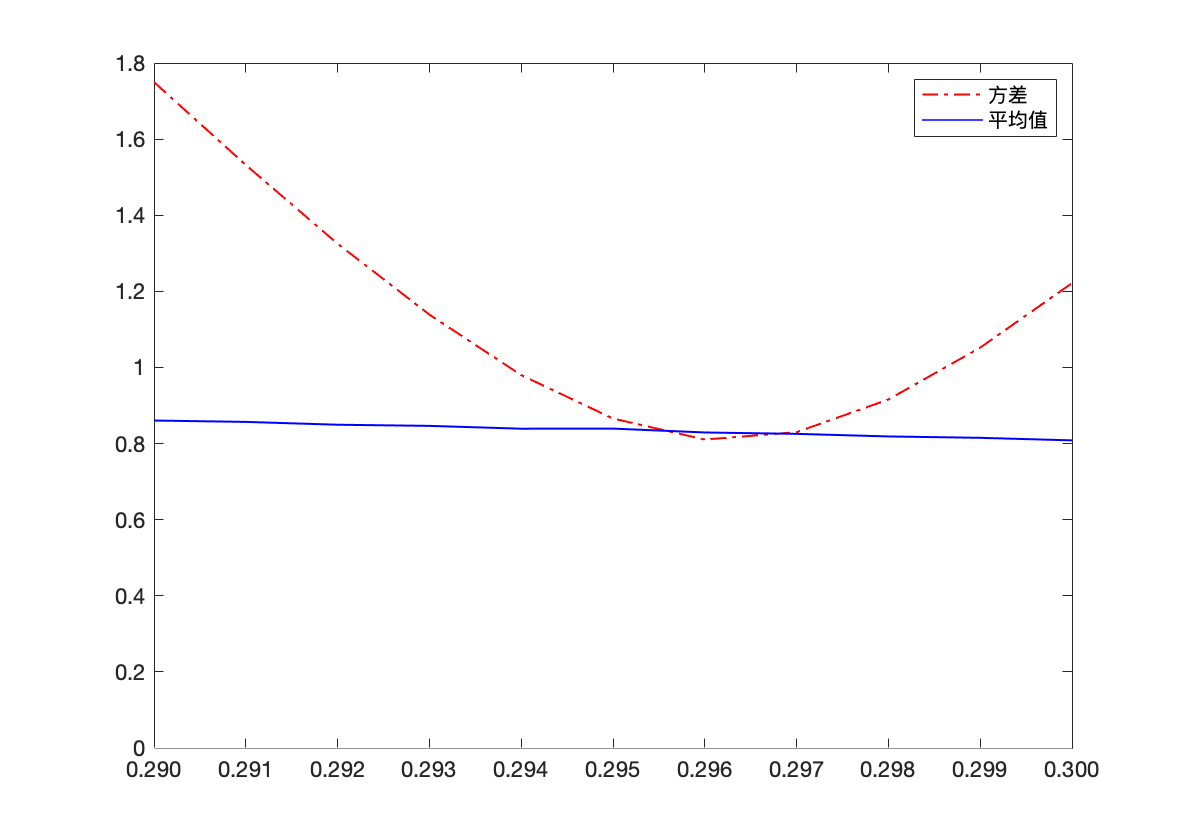
\includegraphics[width=0.8\textwidth]{方差期望.png}
				\caption{$\widetilde{t}\in [0.29ms,0.3ms]$时,高压油管的方差与平均值}
			\end{figure}
			\begin{figure}[!htbp]
				\centering
				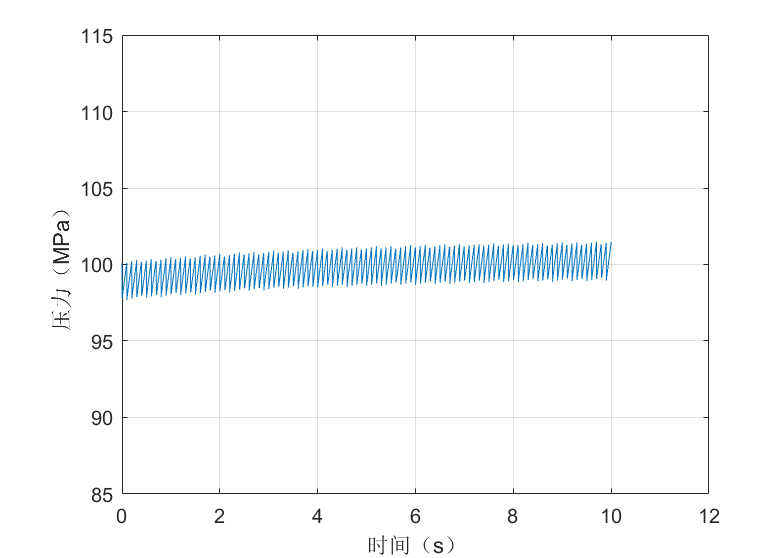
\includegraphics[width=0.8\textwidth]{100稳定.png}
				\caption{$\widetilde{t}=0.296$时,高压油管内压强随时间的变化}
			\end{figure}			
			\subsubsection{情况二:变稳定压强的求解}
			在问题一的第二问中,变换了期望的稳定压强值,要将高压油管内的压力从100MPa增加到150MPa,然后稳定在150MPa。我们设置一个单向阀的时长调整方案。
			调整方案分为两个阶段:
			\begin{itemize}
				\item 第一阶段:增长单向阀开启时长使高压油管在第$i$秒恰好增加到150MPa,$i = 2,5,10$
				\item 第二阶段:缩短单向阀开启时长使高压油管稳定在150MPa
			\end{itemize}
			在第一阶段中,期望找到$\widetilde{t}$使高压油管内的压强在2s、5s或10s时恰好达到150MPa。方程组(8)初始条件任为$t = 0, P_c = 100MPa$。在第二阶段中,期望找到$\widetilde{t}$使高压油管内的压强稳定在150MPa,实际上转换为了情况一的恒定稳定压强的求解,但初始条件为$t = 0, P_c = 150MPa$。
			
			先对简单的第二阶段进行求解,利用5.2.2的方法得到当$\widetilde{t} = 0.76ms$时,高压油管内的压力可以在初始压力为150MPa的条件下,稳定在150MPa。
			\begin{figure}[!htbp]
				\centering
				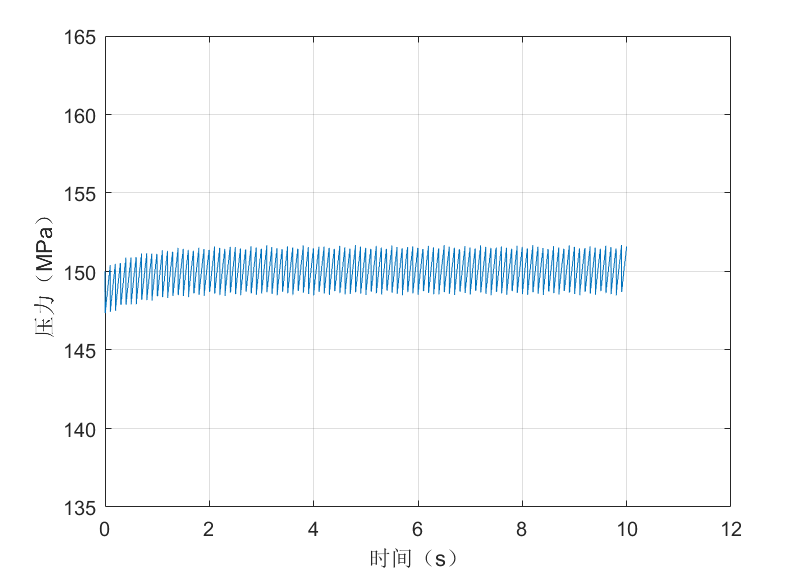
\includegraphics[width=0.8\textwidth]{150稳定.png}
				\caption{$\widetilde{t}=0.76$时,高压油管内压强随时间的变化}
			\end{figure}
			对于第一阶段,对方程组(8)设定条件
			\begin{equation} \left\{
			\begin{aligned}
			&P_c = 150MPa,\ t = 2s/5s/10s \\
			&P_c < 150Mpa,\ t \leq 2s/5s/10s
			\end{aligned}
			\right. \end{equation}
			初值条件为$t = 0, P_c = 150MPa$
			
			用四阶龙格库塔法求解得到当单向阀开启$0.8875s$时,高压油泵在第2秒时恰好达到150Mpa;开启$0.713s$时,在第5秒恰好达到150MPa。然而,我们发现当单向阀至少开启$0.745ms$才能保证高压油管内的压力在稳定时达到150MPa,对于这样的开启时间,在油管工作开始$8s$后就已到达平衡,因此无法通过只增加单向阀开启时间使高压油管内的压力在第10秒时到达150Mpa。因此,通过大量实验我们给出两种方案:
			
			1. 要求10s内到达的方案与要求8s内到达的方案一致
			
			2. 由第二阶段可知,当单向阀开启时长为$0.76s$时,压力能够稳定在150Mpa,那么我们将10s分段,分为增压段与二次增压段。二次增压段时,设置单向阀的开启时间为$0.76s$,就能保证压力在二次增压后稳定在150Mpa。而增压段的持续时长与此时单向阀的开启时长有非常多种组合———只需保证高压油管内压力在第10秒时恰好到达150Mpa即可。
			
			综合上述结果得到以下单向阀调整方案:
			
			
			这样的方案可以非常好地满足变稳定压强情况下的高压油管内压强的稳定。
			\begin{figure}[!htbp]
				\centering
				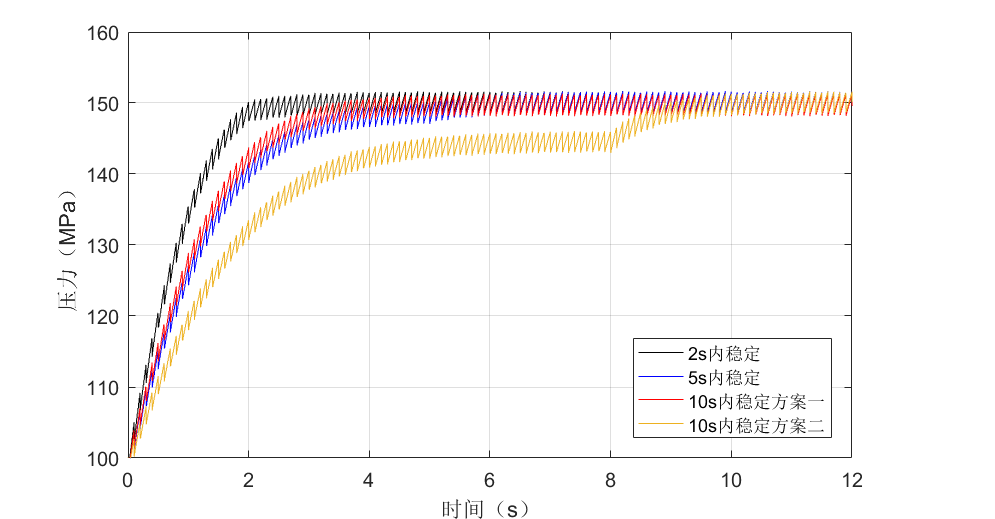
\includegraphics[width=1\textwidth]{方案示意图.png}
				\caption{不同控制方案下高压油管内压强随时间的变化}
			\end{figure}
			\subsection{问题二:泵-管-喷嘴模型}
			在问题二中,考虑了较为复杂的情况,在实际中进入高压油管的燃油来自高压油泵的柱塞腔出口,出口处由一个单向阀与高压油管连接。当单向阀油泵测的压力大于油管测的压力时,单向阀开启;否则,处于关闭状态。高压油管由凸轮驱动,凸轮旋转的快慢决定了油泵柱塞运动的快慢,进而影响其内压强变化。进入高压油泵的燃油仅由油泵内的压强与油管内的压强决定,为了找到使高压油管内压强稳定的凸轮角速度,我们将把高压油泵、高压油管和喷油嘴看作一个系统,研究高压油泵的平均压力与高压油管的平均压力随时间的变化。
			
			根据假设,柱塞与针阀的运动都是周期性的,我们将分别考虑两者运动过程中压力与时间的变化关系。
			\begin{figure}[!htbp]
				\centering
				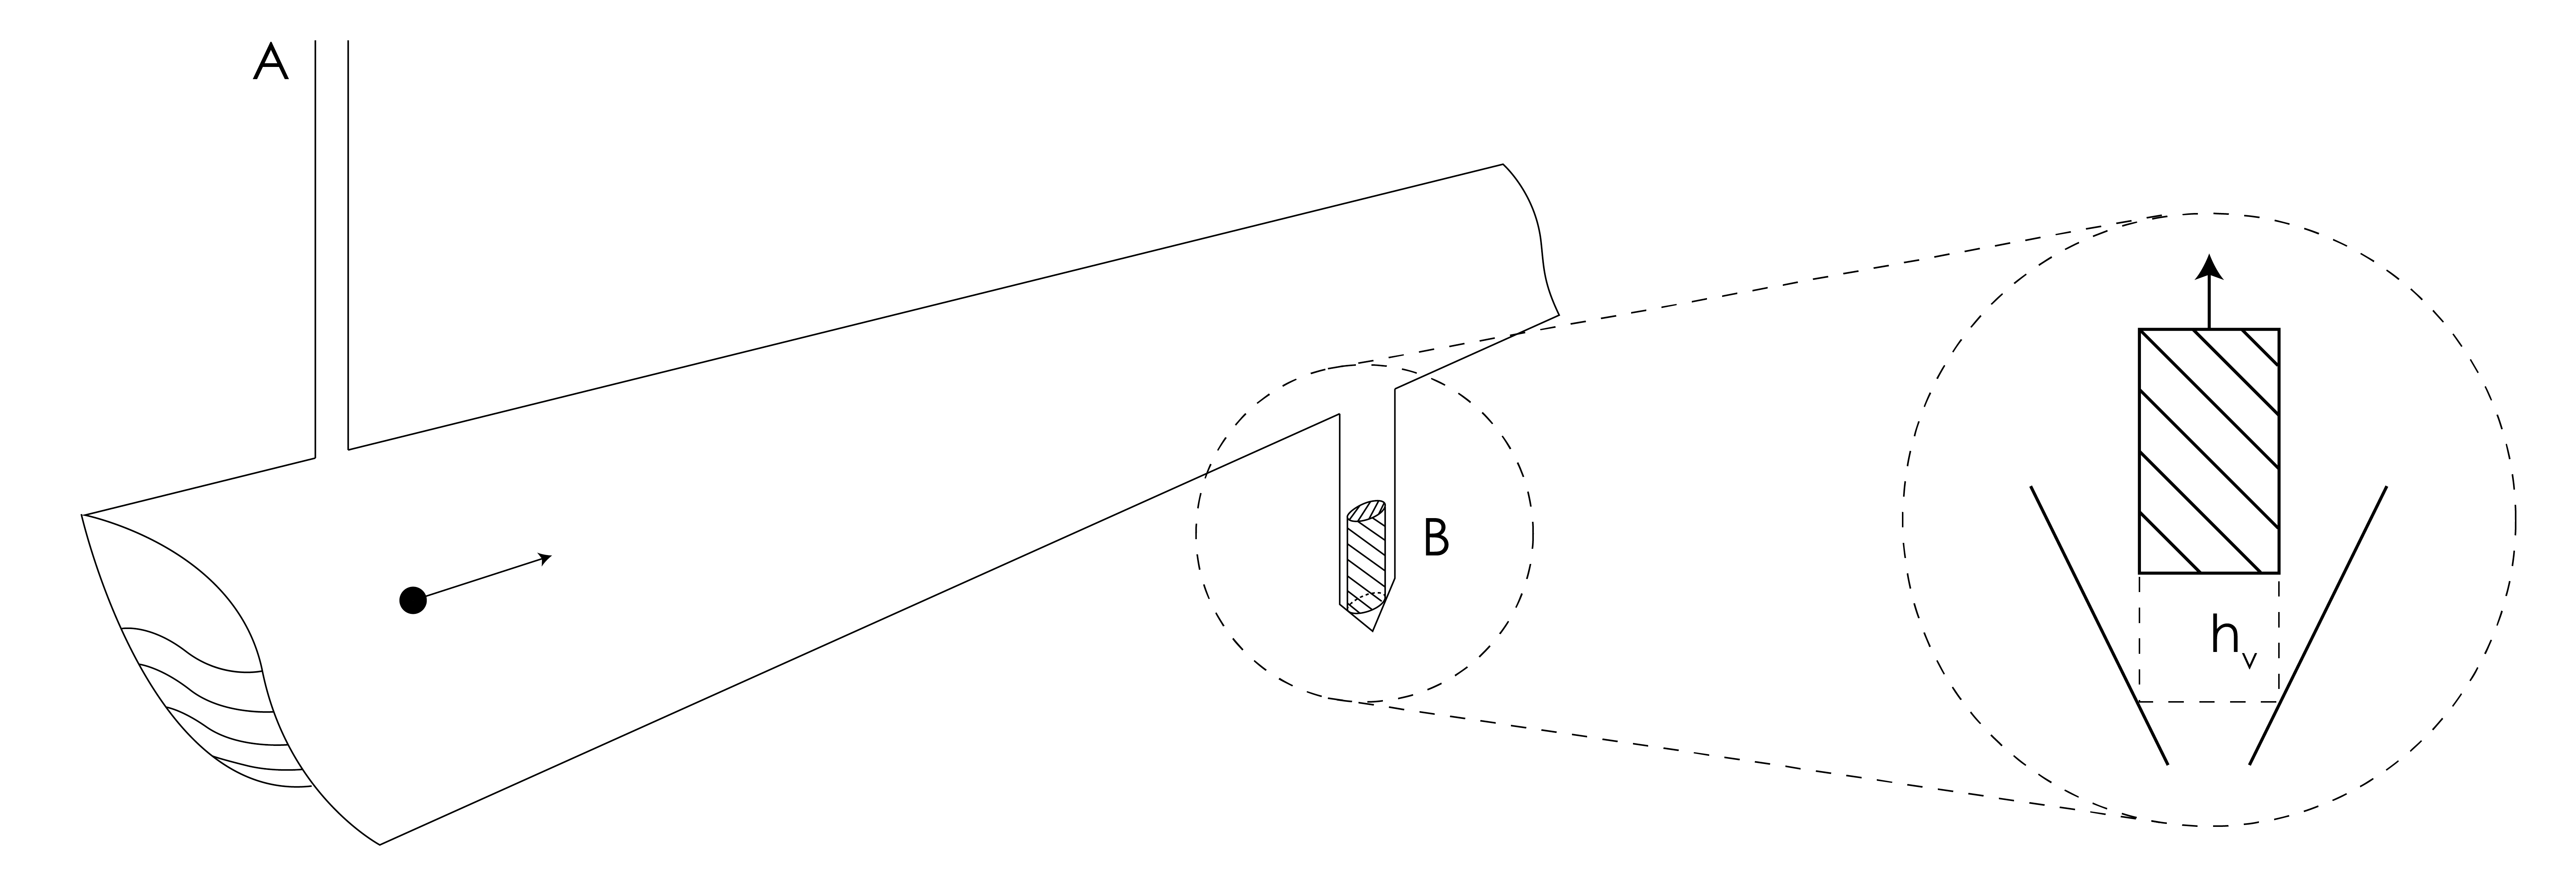
\includegraphics[width=1
				\textwidth]{整体示意图.png}
				\caption{整体示意图}
			\end{figure}
			\subsubsection{柱塞运动过程}
			\begin{figure}[!htbp]
				\centering
				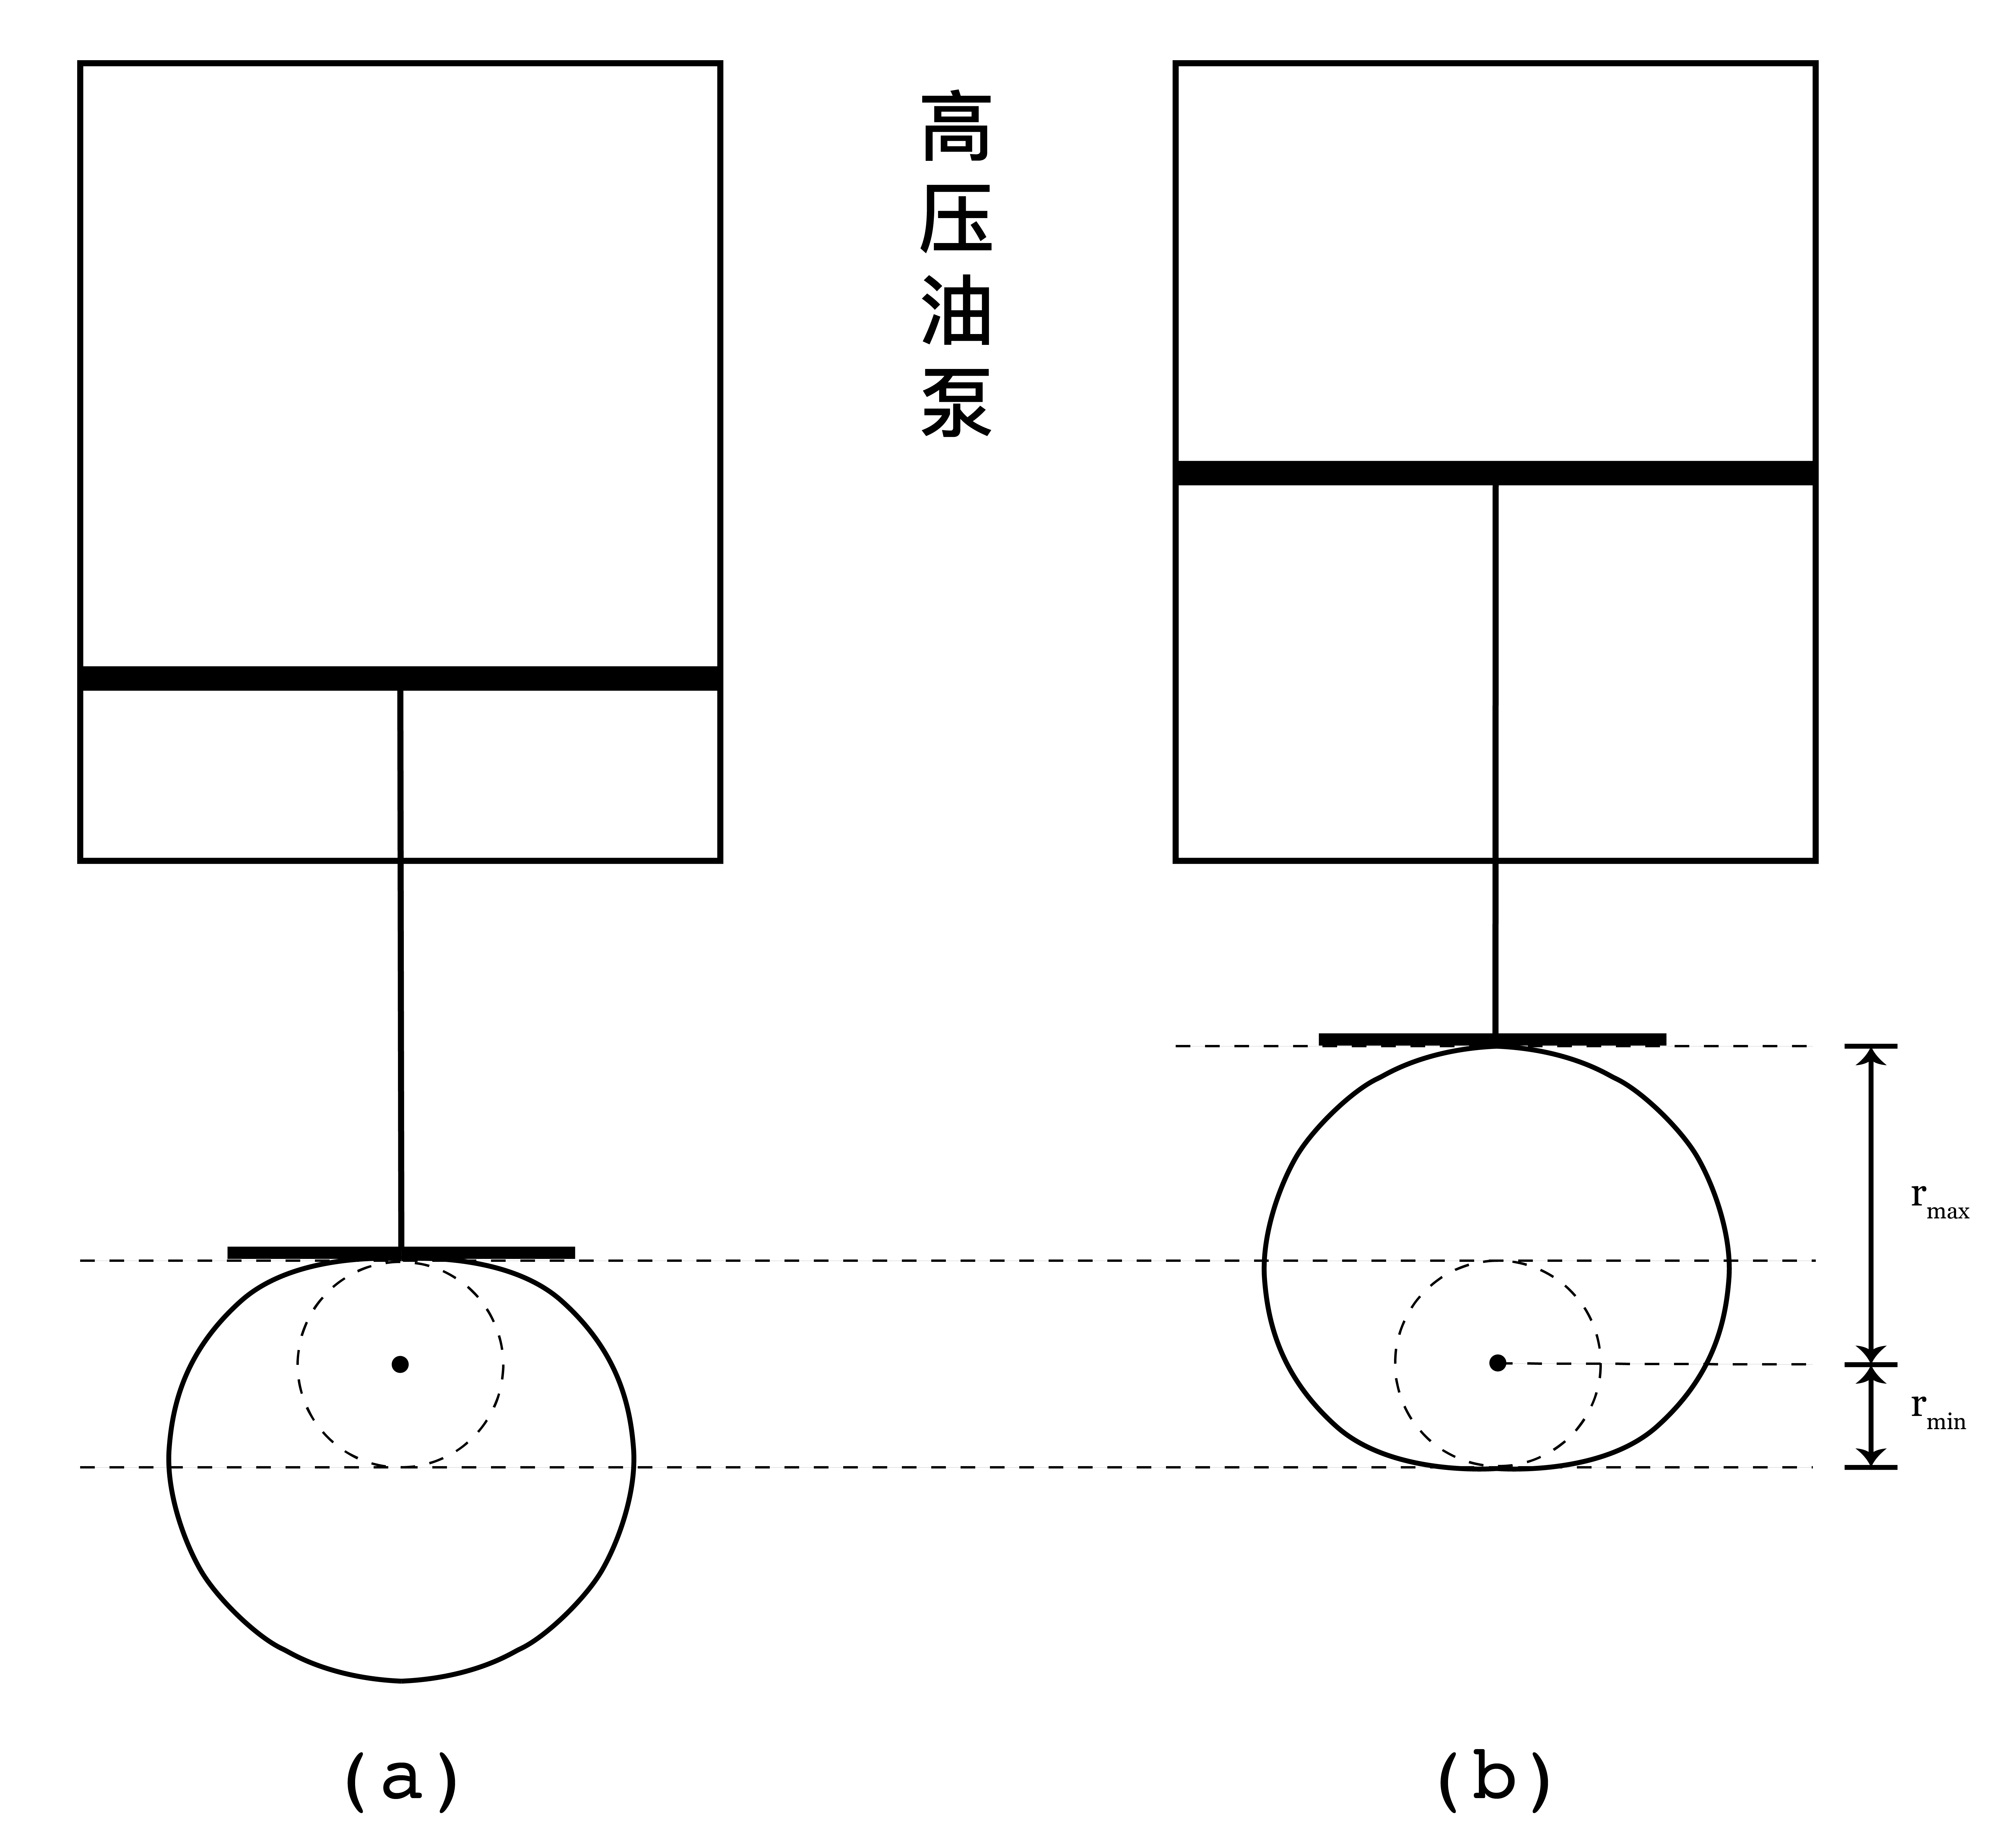
\includegraphics[width=0.8\textwidth]{油泵示意图.png}
				\caption{高压油泵示意图}
			\end{figure}
			
			高压油泵柱塞的压油过程由凸轮驱动柱塞上下运动实现,当挺柱体在凸轮基圆时,如图1(a)所示,柱塞腔与低压油腔通过进、回油孔联通,从而向柱塞腔供油。柱塞向上移动时压缩柱塞腔内的燃油,燃油压强随着体积变小而不断变大,当柱塞腔内的压力大于高压油管内的压力时,柱塞腔与高压油管连接的单向出油阀开启,使燃油进入高压油管内。由于忽略柱塞腔向外的泄露流量及流入低压油道的流量,在$t$至$t + \mathrm{d}t$时刻内,柱塞腔内燃油量的平衡关系由下式给出:
			
			\begin{equation}Q_P = Q_{VP} + Q_{in}\end{equation},高压油泵内的连续性方程由(8)给出:
			
			\begin{equation}\frac{\mathrm{d}P_p}{\mathrm{d}t} = \frac{E}{V_p}(Q_{p} - Q_{in})\end{equation}
			
			其中几何供油率$Q_P$是指喷油泵凸轮随凸轮轴转角$\theta = \omega t$变化而供入系统的燃油流量,它与柱塞升程$h_p$具有以下关系:
			
			\begin{equation}Q_P = A_p \frac{\mathrm{d}h_p}{\mathrm{d}t} = \frac{\pi d_p^2}{4} \cdot \frac{\mathrm{d}h_p}{\mathrm{d}t}\end{equation}
			$A_p$为柱塞横截面积,$d_p$为柱塞的直径。
			柱塞腔有效容积$V_p$也直接取决于柱塞升程:
			
			\begin{equation}V_p = V_0 + A_p (r_{max} - r_{min} - h_p)\end{equation}
			
			\begin{figure}[!htbp]
				\centering
				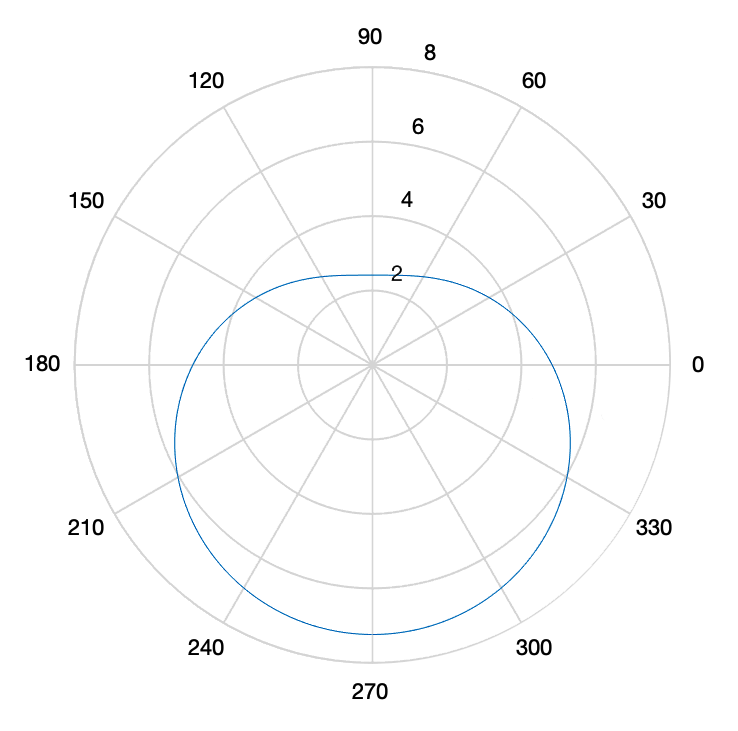
\includegraphics[width=0.5\textwidth]{凸轴示意图.png}
				\caption{凸轴示意图}
			\end{figure}
		
			在极坐标下画出附件二所给的极径与极角的数据,如图7所示,并得到最大极径$r_{max}$与最小极径$r_{min}$。凸轮绕极心旋转,旋转时凸轮最高点与推动柱塞的装置相接,假设接触面光滑,那么柱塞升程$h_p$仅由凸轮的旋转决定。若以凸轮基圆与挺住体接触为初始角,可以通过极坐标转换求出在各幅角离散点上的柱塞升程,利用Fourier逼近得到在一个旋转周期里的近似曲线:
			\begin{equation}h_p = 2.213 - 2.243 \cos(0.8316 \omega t) + 1.341 \sin(0.8316 \omega t)\end{equation}
			
			根据单向阀的运作原理,流入油管的流量可以表达为
			
			\begin{equation}Q_{in} = \xi CA_{in} \sqrt{\frac{2(p_p - p_c)}{\rho_p}} = \xi C \frac{\pi d_{in}^2}{4} \sqrt{\frac{2(p_p - p_c)}{\rho_p}}\end{equation}
			
			其中$\xi = \left\{ \begin{aligned}  1, \, P_p \geq P_c \\ 0, \, P_p < P_c \end{aligned} \right.$模拟了单向阀的开关机制。
			
			另外,$Q_{VP}$代表柱塞腔压力变化引起的压缩油量变化率:
			$$
			Q_{VP} = \frac{V_p}{E} \frac{\mathrm{d}P_p}{\mathrm{d}t}
			$$
			综合(),(),()和()式得到以下关系:
			\begin{equation}
				\frac{\mathrm{d}P_p}{\mathrm{d}t} = \frac{E}{V_p} \left[ \, \frac{\pi d_p^2}{4}  \frac{\mathrm{d}h_p}{\mathrm{d}t} - \xi C \frac{\pi d_{in}^2}{4} \sqrt{\frac{2(p_p - p_c)}{\rho_p}} \, \right]
			\end{equation}
			
			
			
			
			\subsubsection{针阀运动过程}
			
			针阀在高压油管运作时周期性工作,与问题一一致针阀每秒喷油运动10次,当针阀开启高压油管便向外喷油。
			喷油器针阀的运动规律对喷油器的响应时间以及喷油规律起决定性作用,而针阀的升程由附件2(针阀运动曲线 )给出,对数据进行函数拟合,拟合误差为$RMES = $。在一个运动周期内,升程与时间的关系为:
			
			\begin{equation}
			h_v(t) = \left\{ \begin{array}{ll} \begin{array}{ll}
			-799.1 t^5 + 597.2 t^4 - 106 t^3 + 10.21 t^2 \\ -  0.3637 t + 0.002418 \end{array} &, 0 \leq t < 0.45 \\
			2 &, 0.45 \leq t \leq 2 \\
			\begin{array}{ll}
			799.47t^5 - 9194.07 t^4 + 42220.88 t^3 - 96759.84 t^2 \\ + 110643.07 t - 50489.73 
			\end{array} &, 2 < t < 2.46 \\
			0 &, t \geq 2.46
			\end{array} \right.
			\end{equation}
			
			针阀宽度直径大于喷油嘴的直径,只有当$h_v > 0$时,即针阀向上运动,燃油才能向喷孔流动喷出。因此,喷油的有效横截面积取决于针阀的升程,其具体表达式为
			
			\begin{equation}A_{out} = \min\left\{ \pi[d_v h_v(t) \tan \varphi + h_v^2(t) \tan^2\varphi ], \frac{1}{4} \pi d_{out}^2 \right\}\end{equation}
			
			其中$d_{out}$为喷孔直径,向外喷油的流量由喷油嘴两边的压强差与高压油管内的燃油密度决定,而燃油密度随着压强变化而变化,由此可以求出喷出高压油管的流量
			
			\begin{equation}Q_{out} = CA_{out} \sqrt{\frac{2(P_c - P_0)}{\rho_c}}\end{equation}
			
			
			
			\subsubsection{泵-管-喷嘴系统压力变化}
			
			随着柱塞泵的上下运动和喷油等因素的影响,入口体积流量和出口体积流量处于不断变化的状态。根据流体的可压缩性和流动连续性方程,可得到高压油管内燃油压力变化的数学表达式,即
			
			\begin{equation}\frac{\mathrm{d}P_c}{\mathrm{d}t} = \frac{E}{V_c}(Q_{in} - Q_{out}) = \frac{E}{V_c} \left[ \, \xi C \frac{\pi d_{in}^2}{4} \sqrt{\frac{2(P_p - P_c)}{\rho_p}} - CA_{out} \sqrt{\frac{2(P_c - P_0)}{\rho_c}} \, \right]\end{equation}
			
			联立(16),(20)两式得到微分方程组:
			
			\begin{equation} \left\{\begin{aligned}&\frac{\mathrm{d}P_c}{\mathrm{d}t} = \frac{E}{V_c} \left[ \, \xi C \frac{\pi d_{in}^2}{4} \sqrt{\frac{2(P_p - P_c)}{\rho_p}} - CA_{out} \sqrt{\frac{2(P_c - P_0)}{\rho_c}} \, \right] \\&\frac{\mathrm{d}P_p}{\mathrm{d}t} = \frac{E}{V_p} \left[ \, \frac{\pi d_p^2}{4}  \frac{\mathrm{d}h_p}{\mathrm{d}t} - \xi C \frac{\pi d_{in}^2}{4} \sqrt{\frac{2(P_p - P_c)}{\rho_p}} \, \right]\end{aligned}\right. \end{equation}
			
			\subsubsection{模型二模型求解}
			在问题二中,我们期待找到合适的凸轮角速度$\omega$,使微分方程组(20)的解$(P_c,P_p)$满足以下条件:
			\begin{itemize}
				\item $P_c$稳定在100MPa
				\item $P_p$在合理范围内波动
			\end{itemize}
		
			当时间步长取较小值的时候,数值求解计算量巨大,长时间无法得到结果,因此我们选取时间步长$\delta t = 0.1ms$,用四阶龙格库塔法对微分方程组(20)求得数值解。与模型一找最优解的方法类似,我们确定当凸轮角速度为$rad/ms$时,能够满足题目要求,使高压油管内的压强稳定在100MPa。
						
			\subsection{问题三:配置低压阀的泵­-管-­喷嘴模型}
			问题三在泵-管-喷嘴模型的基础上,增加一个与问题一规律相同的喷油嘴和一个单向减压阀。当系统存在两个喷油嘴时,考虑二者同步工作与不同步工作两种情况,分别调整凸轮角速度从而实现高压油管内压力的稳定性。然后考虑增加低压阀的的情况,低压阀的调节使得高压油管腔内压力发生变化,设置低压阀开启与关闭时长,建立新的油管压强方程,改变供油速率从而实现稳定。
			
			\subsection{喷油策略}
			当存在两个喷油嘴时,我们需要考虑喷油嘴是否同时开启,因此为了确定适合的喷油策略,因此我们确定两种方案求解出相对的凸轮角速度,对比得到较好的方案。
			
			\subsubsection{两个喷油嘴同步工作}
			由于喷油嘴的工作特性相同,两个喷油嘴同步工作时喷出高压油管的流量相当于一个喷油嘴流量的两倍。于是,在模型二的基础上稍作调整,根据燃油的可压缩性和流体的连续性方程,微分方程组(20)变换为
			\begin{equation}
				P_c=\frac{E}{V_c}(Q_p-Q{in})
				P_p=\frac{E}{V_p}(Q_{in}-2Q_{out})
			\end{equation}
			
			\subsubsection{两个喷油嘴间隔工作}
			我们设计两个喷油嘴间隔工作时,间隔周期一致。由于每个喷油嘴每秒需要开启10次,两个喷油嘴分开工作相当于一个喷油嘴在每秒需要开启20次。喷油嘴的工作周期从$T = 100ms$变换为$T = 50ms$。于是,微分方程组(20)变换为
			\begin{equation}
			P_c=\frac{E}{V_c}(Q_p-Q{in})
			P_p=\frac{E}{V_p}(Q_{in}-Q_{out})
			\end{equation}
			其中$Q_{out}$中的$T$变为$50ms$。
			1. 两个喷油嘴同步工作
			T=100ms
			2.喷油嘴不同步工作
			T=50ms
			
			配置低压阀的泵­-管-­喷嘴模型的压强变化
			减压阀
			Qd
			
			\section{模型的改进}
			
			\subsection{燃油流动中的压力波传递}
			
			在实际情况下,高压油管中的燃油流动可以视为一维非定常层流,是一种有规则的流动状态。在其流动区域内,燃油的流动过程可以用下列一元不稳定流动方程\cite{bib:five}来描述:
			
			\begin{equation}
			\left\{
			\begin{aligned}
			&\frac{\partial P}{\partial x} + \rho \frac{\partial u}{\partial t} + 2 \rho K u = 0 \\
			&\frac{\partial u}{\partial x} + \frac{1}{a^2 \rho} \cdot \frac{\partial P}{\partial t} = 0
			\end{aligned}
			\right.
			\end{equation}
			式中:$u$为流速;$a$为压力波传递速度(当地音速);$K$为燃油粘性系数;$x$为距离坐标;$t$为时间坐标。
			
			由于本文模型中考虑的是平均压力,我们可以视模型中各腔均为集中容积,不考虑燃油在系统内流动引起的油压传播时间和流动损失,即腔内压力处处相等。然而对于更为复杂的问题,我们可能无法忽略压力波的传递效应。在此情况下,我们需要给定方程组 (21) 的初始条件和边值条件,以求出高压油管中任意时刻任意位置的速度和压力。
			
			\subsection{模型求解的改进}
			
			在模型求解的过程中,我们分别遇到了常微分方程和方程组的数值求解问题。对于问题一,我们取四阶龙格库塔算法的迭代步长为0.01;对于问题二、三,我们取ode15s函数的迭代步长为0.01。由于微分方程数值求解的精度直接取决于迭代次数,迭代步长越小,计算结果将更精确。但受限于程序运行时间,我们仅将步长定为0.01。
			
			\section{模型的优缺点}
			\subsection{模型的优点}
			
			\subsection{模型的缺点}
			模型二的求解复杂程度明显大于模型一,微分方程组(20)在四阶龙格库塔法求解的每一步迭代中计算量明显比微分方程(8)大得多。对于求解效率而言,四阶龙格库塔法计算量大,计算时间长,所耗内存空间大,不利于在短时间内做大量实验,特别是对模型二这样的复杂方程组更是如此。我们在模型二的求解过程中选取时间步长为$0.1ms$,由于在该系统内,喷油嘴与单向阀的周期都为微秒级别,因而这样的时间步长导致的误差值偏大。
			
			
			%参考文献
			\begin{thebibliography}{9}%宽度9
				\bibitem{bib:one} 蔡梨萍. 基于MATLAB的柴油机高压喷油过程的模拟计算[D].华中科技大学,2005.
				
				\bibitem{bib:two}李旭林,何勇灵.两相条件下柴油机喷油系统的数学模型[J].内燃机学报,2007(05):428-432.
				
				\bibitem{bib:three}Lino, Paolo \& Maione, Bruno \& Rizzo, Alessandro. (2005). A control-oriented model of a Common Rail injection system for diesel engines. IEEE International Conference on Emerging Technologies and Factory Automation, ETFA. 1. 7 pp. - 563. 10.1109/ETFA.2005.1612572. 
				\bibitem{bib:four}朱婉. 基于Simulink的柴油机高压共轨喷油系统建模与仿真[D].合肥工业大学,2015.
				\bibitem{bib:five}约翰D.安德森(美).计算流体力学基础及其应用[M].机械工业出版社,2007:29-31.
				
			\end{thebibliography}
			
			\newpage
			%附录
			\appendix
			\section{主程序--matlab 源程序}
			\begin{lstlisting}[language=matlab]
			function [dist,xiane,xinyuzhi] = clac()
			info_renwu = load('renwu_information.txt');
			row = size(info_renwu,1);
			col = size(info_renwu,2);
			dist = zeros(row,1);
			xiane  = zeros(row,1);
			xinyuzhi = zeros(row,1);
			dingjia = info_renwu(:,3);
			for i = 1:row
			[dist(i),xiane(i),xinyuzhi(i)]=variable(info_renwu,i); 
			end
			
			\end{lstlisting}
			
			\section{计算距离--matlab 源程序}
			\begin{lstlisting}[language=matlab]
			function dis = distance(wei1,jing1,wei2,jing2)
			R = 6370;
			%dis = asin(sqrt(sin((wei1-wei2)/2)^2+cos(wei1)*cos(wei2)*sin((jing1-jing2)/2)^2));
			%dis = dis*2*R;
			dis = 2*pi*R/360*((wei1-wei2)^2+(jing1-jing2)^2*cos((wei1+wei2)/2)^2)^0.5;
			
			\section{聚类--matlab 源程序}
			\begin{lstlisting}[language=matlab]
			function [dist,xiane,xinyuzhi] = variable(info_renwu,i)
			info_huiyuan = load('huiyuan_location.txt');
			data_xiane = info_huiyuan(:,3);
			data_xinyu = info_huiyuan(:,4);
			data_wei = info_huiyuan(:,1);
			data_jing = info_huiyuan(:,2);
			num = size(data_jing,1);
			data_distance = zeros(num,1);
			sum = 0;
			for j = 1:num
			data_distance(j) = distance(info_renwu(i,1),info_renwu(i,2),info_huiyuan(j,1),info_huiyuan(j,2));
			end
			[a,b] = sort(data_distance);
			first = b(1:30,:);
			for count = 1:30
			sum = sum + data_distance(first(count));
			end
			dist = sum/30;
			sum = 0;
			for count = 1:30
			sum = sum + data_xiane(first(count));
			end
			xiane = sum/30;
			sum = 0;
			for count = 1:30
			sum = sum + data_xinyu(first(count));
			end
			xinyuzhi = sum/30;
			
			\end{lstlisting}
			
			
			
			
			
			
		\end{document} 
